\chapter{Freestyle \& Standard Skill \label{chap:freestyle} Overview}

\section{The Difference Between These Events}
In Standard Skill, riders demonstrate pure skill and mastery on a standard unicycle, by performing up to 18 skills they have pre-selected.
Standard Skill judging is based on the point value of the skills and quality of their execution, not the `show.' In Freestyle, riders perform to music, with costumes, props and any kinds of unicycles.
Riders are judged not only on skill, but also on how well they entertain and put on a show.
There are Individual, Pair, and Group Freestyle events.

\section{Age Groups}
\textbf{Note:} Age groups may be different for different types of event.
The minimum allowable age groups are listed for each event.
Convention hosts are free to add more age groups.
Age group is determined by the rider's age on the first day of the convention.
Junior Expert is open to all riders 0-14.
Expert is open to riders of any age, including 0-14.
Riders must state the age group in which they are entering for each artistic event in which they participate.

\textbf{Example:} Riders who enter Individual Freestyle as Experts can enter Pairs in their age group if they wish.
Riders are divided male/female in Standard Skill and Individual Freestyle, but not in Pairs or Group.

\subsection{Riders Must Be Ready}
Riders who are not ready at their scheduled performance time may or may not be allowed to perform after the last competitor in their age group.
The Chief Judge will remember to consider language barriers, and that riders may be engaged in convention work to slow them down.
Except for Standard Skill, a rider may not perform before a different set of judges than those that judged the rest of their age group.

\section{Safety Gear}
No safety gear is needed.

\section{Performance Set-Up}
Competitors are allowed a maximum of two minutes to set up their unicycles and props in the performing area.
Competitors who take too long risk being disqualified.
An extension of the set-up time can be given only by the Chief Judge and must be requested in advance.
Competitors must show a legitimate need when requesting more time, such as numerous props or complicated special effects.

\section{Interruption Of Judging}
An interruption of judging can result from material damage, injury or sudden illness of a competitor, or interference with a competitor by a person or object.
If this happens, the Chief Judge determines the amount of time left and whether any damage may be the fault of the competitor.
Re-admittance into competition must happen within the regulatory competition time.
If a routine is continued and the competitor was not at fault for the interruption, all devaluations coming forth from the interruption will be withdrawn.

\section{Music \label{sec:freestyle_music}}
In Freestyle events, music is included in the judging and competitors should use it.
In Standard Skill music is not judged.
But background music will be provided during all Standard Skill routines, or competitors may provide their own.
Competitors may also, at their request, have no music played.
It is recommended to have one or more backup copies of all music in case of loss or damage.
For recordable disks, competitors are also recommended to test their music on multiple players to make sure it will work at competition time.

\subsection{Media Types}
The host is required to have the capability of playing recordable CDs.
Other media types may also be supported, at the host's discretion.
The Artistic Director is responsible for announcing what media types will be supported, and making sure the necessary equipment is provided.

\subsection{Music Preparation}
Competitors must provide their music in a type that is supported, and has been announced by the Artistic Director.
All music must be clearly labeled with the competitor name(s), age group, event type (such as Pairs), and if needed, the track number.
Whenever possible, competition music should be the first track on the CD.
The DJ (music operator) is not responsible for any errors resulting from unsupported types or mislabeled tracks.

\subsection{Music Volume}
Volume level is controlled by the DJ, at instructions from the Chief Judge.
The base volume for Freestyle music should be loud enough to sound clear, and be heard by all.
For Standard Skill, volume level should not be loud enough to interfere with judge communication, but otherwise similar to the level for Freestyle.
Some competitors' music may start with especially loud or quiet sections, and the DJ should be advised of these so volume levels do not get compensated in the wrong direction.
Some competitors may request that their music be played at lower levels.
These requests can be made directly to the DJ.
Requests for higher volumes must be approved by the Chief Judge, who has the option of passing this responsibility to the DJ.

\subsection{Special Music Instructions}
Some competitors may have special music instructions, such as stopping or starting the music at a visual cue, changing volume level during the performance, etc.
The DJ is not responsible for errors carrying out these instructions.
For best results, the competitor should supply a person to coach the DJ during the performance, so there are no mistakes.
If the DJ receives instructions that sound unusual, the Chief Judge should be consulted for approval.

\section{Announcing Of Results}
Final results will be continuously announced and/or posted for public view.
Results Sheets will be posted after each age category of an event.
The protest period begins at this point.

\section{Protests}
Must be filed in writing, within 15 minutes from the posting of event results.
Protest against judges' scores is not permissible.
Protest is only possible against calculation mistakes or other mistakes not connected to the scoring.
The Chief Judge must resolve all protests within 30 minutes from receipt of the written form.

\section{Freestyle Judging Panel \label{sec:freestyle_judging-panel}}
There are five (or more) judges each of Technical and Presentation for Age Group competitions; five (or more) judges each of Technical and Presentation for Jr. Expert and Expert competitions (including Group).
All judges must attend a workshop provided as part of the convention schedule before the start of the Freestyle competitions.
Exceptions to workshop attendance are granted by the Chief Judge if judging rules have not changed since the previous judging experience and the judge has high Accuracy Scores.
Unless otherwise noted, judges at a Unicon must either speak English or have translation assistance for the specified language while judging.
Judges at other unicycle conventions should speak the dominant language of that convention or have translation assistance.

Judges' names must be provided to the Chief Judge (via email, FAX, or postal mail) by at least one month prior to the start of the unicycle convention and include the number of freestyle conventions where they have been a competitor, judge, or simply in the audience.
See section \ref{subsec:freestyle_judging-panel_nominating-freestyle-judges} for description of which teams/countries are required to provide judges.
Judges must be at least 15 years of age at the start of the event.
Judges are recommended to be a current freestyle competitor, a former freestyle competitor, an active coach of freestyle routines, a proven judge at prior competitions, or an avid spectator who has observed many freestyle routines.
Details about the Standard Skill judging panel are covered in section \ref{sec:freestyle_std-judging-panel}.

\subsection{Selecting Judges \label{subsec:freestyle_judging-panel_selecting-judges}}
A person should not judge an event if he or she is:
\begin{itemize}
\item A parent, child or sibling of a rider competing in the event.
\item An individual or team coach, manager, trainer, colleague who is member of the same club specified in the registration form, colleague's family etc.
of a rider competing in the event.
\item More than one judge from the same family judging the same event at the same time.
\end{itemize}
If the judging pool is too limited by the above criteria, restrictions can be eliminated starting from the bottom of the list and working upward as necessary only until enough judges are available.
If there are some candidates who have the same level of restrictions and judging score, their agreement about publishing the results need to be considered.
The eliminations must be agreed upon by the Chief Judge and Artistic Director, or next-highest ranking artistic official if the Chief Judge and Artistic Director are the same person.

\subsection{Assignment Of Age Group Judges}
Judges will be chosen from the list of judges as provided in section \ref{subsec:freestyle_judging-panel_nominating-freestyle-judges}.
Judges who are competing in the event just before or just after the current category are eliminated from the list.
Judges will also be eliminated from the list for the current category as described in section \ref{subsec:freestyle_judging-panel_rating-judge-performance}.
The final selection of judges will be chosen based on their accuracy scores from the remaining list.

\subsection{Assignment Of Expert (And Junior Expert) Judges \label{subsec:freestyle_judging-panel_assignment-of-expert-judges}}
Assignments for Expert and Jr. Expert judges will be made by the Chief Judge using the most qualified of all judges available.
Qualifications are determined in the following order of importance: 
\begin{itemize}
\item Highest judging accuracy scores obtained while judging age group (age groups judges must have a minimum of five entrants) or other Jr. Expert and Expert events.
\item Greatest amount of Jr. Expert and Expert judging experience.
\item Greatest amount of international judging experience.
\item Greatest number of Freestyle competition experienced (viewed, judged, or as a competitor).
\end{itemize}
Judges who are competing in the event just before or just after the current category are eliminated from the list.
Judges will also be eliminated from the list for the current category as described in section \ref{subsec:freestyle_judging-panel_selecting-judges}.
Judges will also be eliminated from the list if they exhibit Judging weaknesses during their Age Group judging as described in Section \ref{subsec:freestyle_judging-panel_rating-judge-performance}.
At Unicons, if more than five judges each of Technical and Presentation remain, judges who have not judged at a previous Unicon will be removed from the list.
If there are still more than five each then the final list of judges for the category will be chosen by accuracy scores as defined in section \ref{subsec:freestyle_judging-panel_calculating-accuracy-scores}.

\subsection{Judging Panel May Not Change}
The individual members of the judging panel must remain the same for entire age groups; for example one judge may not be replaced by another except between age groups.
In the event of a medical or other emergency, this rule can be waived by the Chief Judge.

\subsection{Rating Judge Performance  \label{subsec:freestyle_judging-panel_rating-judge-performance}}
Judges are rated by comparing their scores to those of other judges at previous competitions.
Characteristics of Judging Weaknesses
\begin{itemize}
\item \textbf{Excessive Ties:} A judge should be able to differentiate between competitors.
Though tying is most definitely acceptable, excessive use of tying defeats the purpose of judging.
\item \textbf{Group Bias:} If a judge places members of a certain group or nation significantly different from the other judges.
This includes a judge placing members significantly higher or significantly lower (a judge may be harsher on his or her own group members) than the other judges.
\item \textbf{Inconsistent Placing:} If a judge places a large number of riders significantly different from the average of the other judges.
\end{itemize}

\subsection{Re-Instating Judges}
If a judge has been labeled as having a Judging Weakness, they may have a chance to be re-instated on the list by:
\begin{itemize} 
\item Discuss with the Chief Judge the scores that were Tied, Biased, or Inconsistent.
\item Practice judge on at least two categories with at least 4 competitors.
\end{itemize}
If the practice judging shows no further examples of Judging Weakness, they may be reinstated on approval by the Chief Judge and Artistic Director.
If the Chief Judge and Artistic Director are the same person, then the next highest-ranking official must agree to the reinstatement.

\subsection{Calculating Accuracy Scores \label{subsec:freestyle_judging-panel_calculating-accuracy-scores}}
The Chief judge should decide to replace a judge if he/she shows signs of weakness.
To find the right decision, the chief judge may use heuristics, statistical analytics, etc. as indicators.

\subsection{Nominating Freestyle Judges \label{subsec:freestyle_judging-panel_nominating-freestyle-judges}}
Parties (Countries/Clubs) that participate at competitions must nominate judges in relation to the number of Freestyle participants they send (see table below). 
After registration finishes, the chief judge will send a request to all parties.
The request contains the compiled number of minimum judges per party and a question to nominate the candidates.
Judge nominations include the experience of the judges (such as previous competitions, how long he/she has been judging, agegroup/expert judging or other relevant qualifications such as educations).

\begin{tabular}{|l|l|}
\hline
\textbf{Number of Participants per Party} & \textbf{Minimum Number of Judges per Party} \\
\hline
$<$5 & 0 \\
\hline
5-10 & 2 \\
\hline
11-20 & 3 \\
\hline
21-30 & 4 \\
\hline
$>$30 & 5 \\
\hline
\end{tabular}

\subsection{Not Providing Judges}
At Competitions, parties that are unable to provide their required number of judges (either Group or Individual/Pairs) may have their competitors removed from that competition.
Exceptions will be granted on a special basis with a letter to the Chief Judge, Artistic Director, and Convention Director. 
\textbf{Note:} A party that isn't able to nominate their minimum judges can ask a party that has more than the required number of minimum judges to nominate their additional judges as their own.

\subsection{Judges Workshop}
The hosts of the convention must provide for a judge's workshop at least 24 hours prior to the start of the Freestyle competition.
A minimum of 3 hours must be set aside, in a classroom or similar environment.
If possible, it is strongly recommended to have more than one workshop to accommodate schedules.
Variations on this can be approved by the Chief Judge.
Workshop schedule(s) must be announced to all judges at least three weeks prior to the start of the competition.

Judges should have read the rules prior to the start of the workshop.
The workshop will include a practice judging session.
Each judge will be required to sign a statement indicating they have read the rules, attended the workshop, agree to follow the rules, and will accept being removed from the list of available judges if their judging accuracy scores show Judging Weaknesses.

\section{Scoring}
In all events except Standard Skill, the scores of each judge are transferred into placing points, which represent the ranking of each competitor by that judge.
The highest scoring competitor gets 1 placing point, the next one gets 2, and so on.

\textbf{Note:} The ranking number, or highest placing point available for a competitor depends on the number of entries in that category.
If two or more competitors have the same score, they are awarded equal portions of the total number of placing points available for the places they occupy in the ranking.

\textbf{Example:} Seven competitors.
Four of them tie for 2nd place.
7th place gets 7 points, 6th place gets 6 points, and 1st place gets 1 point.
For the other four competitors, add up the other placing points numbers: $2+3+4+5=14$.
Divide this by the number of competitors (4) to get 3.5 placing points each.

\subsection{Removing The High And Low}
After determining placing points as above, discard the highest and lowest placing score for each rider.
If Rider A has scores of 1,2,1,3,2, take out one of the ones, and the three.
Then Rider A has 1,2,2, for a total of 5.
If Rider B has scores of 2,2,2,2,2, he will end up with 2,2,2, a total of 6.
The winner is the competitor with the lowest total placing points score after the high and low have been removed.

\subsection{Ties}
If more than one competitor has the same placing score after the above process, those riders will be ranked based on their placing scores for Technical.
The scoring process must be repeated using only the Technical scores for the tied riders to determine this rank.
High and low placing scores are again removed in the process.
If competitors' Technical ranking comes out equal, all competitors with the same score are awarded the same place.

\section{World Champions \label{sec:freestyle_world-champions}}
Winners in the Expert category of each event are the \textbf{World Champions}.
In the individual events, separate titles are awarded for male and female.
Winners in the Jr. Expert category are the \textbf{Junior World Champions}.

\chapter{Freestyle Rules}

\section{Individual Freestyle Overview}

\subsection{Minimum Age Groups}
 0-14, 15-UP, Expert.
The decision to enter as Expert or Jr. Expert is optional, but must be stated in advance.

\subsection{Time Limits}
2 minutes for riders 0-14 (except Jr. Expert), 3 minutes for all other age groups (except Expert).
Jr. Expert has a maximum of 3 minutes and Expert has a maximum of 4 minutes.

\subsection{Unicycles}
Any type and any number.

\subsection{Music and Costume}
All are judged, and must be considered in the performance.

\subsection{Props and Decorations \label{subsec:freestyle_freestyle-rules_individual-freestyle-overview_props-and-decorations}}

\textbf{Props} are all items which are used by the rider in his/her performance and require a technical handling by the rider (for example typical objects like clubs, ribbons, hoop, etc.). 
These items can be used to do a unicycling trick, like rope skipping with the unicycle.
However, they can also be employed to show a non-unicycling skill which supports and enhances the choreography, like the elaborate use of a hat.
Props have to be presented by the rider.
It is not mandatory to include props in the performance.
If none are used, the score will not be lower. 

\textbf{Decoration:} In contrast to props, decoration is used to present the rider or clarify the theme of the performance.
Decoration does not require a technical handling by the rider.
For example other persons in costumes and background images.
Decoration is no personal contribution of the rider and therefore effects of the Decorations should not be judged.
On the contrary, Decorations can also be judged negatively if it distracts from the rider's performance.
For Junior Expert and Expert categories at Unicon, it is forbidden to use decorations (including people) that are too large, which the competitor cannot carry and/or put on by oneself. 

For Props and Decoration neither fire nor sharp objects (such as juggling knives) are allowed.

\subsection{Judging Method}
Riders' scores are divided into two parts called Technical and Presentation, each receiving 50\% of the score.
Read the Freestyle Judging section to learn more.

\subsection{Maximum Number of Competitors for Jr. Expert and Expert}
\textbf{Non-Unicon:} Organizers of non-Unicon events can choose to limit the number of competitors using the guidelines below or have no limit.

\textbf{Unicon:} Each country can submit a maximum of three individuals in each category to compete at Unicon in the Individual Freestyle events (three in Jr. Expert Male, three in Jr. Expert Female, three in Expert Male, three in Expert Female).
If a country has placed 1st, 2nd, or 3rd in Individual Freestyle at the previous Unicon, they can submit one additional competitor for each placing in that category.
For example, if Country-A wins first place in Expert Male at the previous Unicon, they may submit up to four individuals for Expert Male at the current Unicon.
If Country-B wins second and third place in Jr. Expert Female at the previous Unicon, they may submit up to five individuals in Jr. Expert Female at the current Unicon.

\subsection{Method for Limiting the Competitors at Unicon}
A country that wishes to submit more than their allocated number of individuals should select individuals by their own way.
Any type of competition using the IUF judging methods to determine their competitors is recommended.
If a country is unable to hold a competition, a country can choose individuals by their own rating method.
For example, if a country has placed 1st, 2nd or 3rd in Individual Freestyle at the previous Unicon, it can give these individuals a higher rating, because they brought additional number of individuals to a country.
If a country did not place in the top three, it can give only the highest placing individual a higher rating.
It is strongly recommended to complete the selection at least three months prior to the start of the Unicon.
If a country cannot select by then, the method and schedule of the selection must be communicated to the Chief Judge and Artistic Director at least three months prior to the start of the Unicon.

\section{Pairs Freestyle Overview}

\subsection{Minimum Age Groups}
Age group (all ages), Expert.
Each rider may enter only once.
The age group of the older rider is the age group for the pair.
Expert is treated as the ``oldest'' age group, followed by Jr. Expert, and then all other age groups.
The decision to enter as Expert or Jr. Expert (if used) is optional, but must be stated in advance.

\subsection{Time Limits}
Same as Individual Freestyle.

\subsection{Unicycles}
Any type and any number.

\subsection{Music and Costume}
Same as Individual Freestyle.

\subsection{Props and Decorations}
Same as Individual Freestyle.

\subsection{Judging Method}
Same as Individual Freestyle, 50\% for Technical, and 50\% for Presentation.
In Pairs, there is extra emphasis on teamwork; two person skills, etc.
(see Judging Criteria).

\subsection{Maximum Number of Competitors for Jr. Expert and Expert}
\textbf{Non-Unicon:} Organizers of non-Unicon events can choose to limit the number of competitors using the guidelines below or have no limit.

\textbf{Unicon:} Each country can submit a maximum of three pairs in each category to compete at Unicon in the Pairs Freestyle events (three in Jr Expert Pairs, three in Expert Pairs).
If a country has placed 1st, 2nd, or 3rd in Pairs Freestyle at the previous Unicon, they can submit one additional competitor for each placing in that category.
For example, if Country-A wins first place in Expert Pairs at the previous Unicon, they may submit up to four Pairs for Expert Pairs at the current Unicon.
If Country-B wins second and third place in Jr Expert Pairs at the previous Unicon, they may submit up to five pairs in Jr Expert Pairs at the current Unicon.
If a pairs team is submitted consisting of members from two countries, that team must choose one of their two countries to represent.

\subsection{Method for Limiting the Competitors at Unicon}
A country that wishes to submit more than their allocated number of pairs should select competitors by their own way.
Any type of competition using the IUF judging methods to determine their competitors is recommended.
If a country is unable to hold a competition, a country can choose pairs by their own rating method.
For example, if a country has placed 1st, 2nd, or 3rd in Pairs Freestyle at the previous Unicon, it can give these pairs a higher rating if BOTH partners from the previous Unicon still be pairs, because they brought additional number of pairs to a country.
If a country did not place in the top three, it can give only the highest placing pairs a higher rating.
It is strongly recommended to complete the selection at least three months prior to the start of the Unicon.
If a country cannot select by then, the method and schedule of the selection must be communicated to the Chief Judge and Artistic Director at least three months prior to the start of the Unicon.

\section{Group Freestyle Overview}
Group freestyle is divided in Big Groups and Small Groups 
Each rider may enter each category (Small Group, Big Group) only once. For example: a rider can be in one small group routine and one large group routine but not two small group routines (without permission).

A rider may appear in a second Group Freestyle performance (Small Group, Big Group) with permission of the Chief Judge, to replace a rider due to illness, injury or other mishap. 

\subsection{Small Group}
Minimum of three riders, maximum of eight.

\subsection{Big Group}
Minimum of nine riders, no maximum number of riders.

\subsection{Minimum Age Groups}
None.

\subsection{Time Limit}
Six minutes.

\subsection{Unicycles}
Any type and any number.

\subsection{Music and Costume}
Same as Individual Freestyle.

\subsection{Props and Decoration}
Same as Individual Freestyle.

\subsection{Juding Method}
Same as Individual Freestyle, but with additional emphasis on teamwork and multiple person skills, such as formation riding.
Extra consideration will be given to account for widely different group sizes, relative skill levels, and relative ages of riders.

\subsection{Maximum Number of Competitors for Jr. Expert and Expert}
\textbf{Non-Unicon:} Organizers of non-Unicon events can choose to limit the number of small/big groups using the guidelines below or have no limit.

\textbf{Unicon:} Each country can submit a maximum of three groups to compete at Unicon in each of the following categories: Expert Small Group, Jr. Expert Small Group, Expert Big Group, and Jr. Expert Big Group.

\subsection{Method for Limiting the Competitors at Unicon}
A country that wishes to submit more than their allocated number of groups should select groups by their own way.
Any type of competition using the IUF judging methods to determine their groups is recommended.
If a country is unable to hold a competition, a country can choose groups by their own rating method.
For example, if a country has placed 1st, 2nd, or 3rd in Group Freestyle at the previous Unicon, it can give these groups a higher rating, because they brought additional number of groups to a country.
If a country did not place in the top three, it can give only the highest placing groups a higher rating.
Not all members from the previous Unicon are required to be members of a new group.
It is strongly recommended to complete the selection at least three months prior to the start of the Unicon.
If a country cannot select by then, the method and schedule of the selection must be communicated to the Chief Judge and Artistic Director at least three months prior to the start of the Unicon.

\section{Deadline For Signing Up}
These events have a deadline for entry, which must be specified in the registration form.
If not specified in the registration form, the deadline is one month before the official convention start date.
A maximum of ten Individuals, ten Pairs routines, and two groups will be allowed to be added after this time to account for difficulties in travel planning or other valid reasons that are communicated about in advance.
These will be added in the order of their request to the Chief Judge and Convention Director via email or fax.
Participants who attempt to sign up less than 36 hours prior to the beginning of the specified competition will not be allowed to enter.
Changing Pairs partners is allowed up to 36 hours prior to the actual competition as long as the category does not change.
Adding or subtracting the members of a group routine is allowed up to 36 hours prior to the start of that competition.

\section{Size Of Performing Areas}
The minimum size for Freestyle event must be 28m x 15m.
Hosts shall give additional space to riders.
Hosts must publicize the dimensions of the available performing area as far in advance of the competition as possible, and organizers of international championships at least three months prior to the event.

\section{Order Of Performance}
Performance order for Jr. Expert and Expert in Pairs/Individual/Group freestyle are defined by an open drawing without a computer.
The drawing/selection should be done publicly and transparently, at a time that is pre-announced, so people can witness it.
The method to determine performance order for age groups is completely up to the Artistic Director.

\section{Start Of Performance}

\subsection{Freestyle Events}
The judging, the stopwatch, and the `performance' all start at the same time.
The Timer starts the watch at the beginning of the music, or at a signal from competitors, whichever comes first.
The signal can be a nod, wave, bow, verbal cue (``Start!'') or any clearly understandable means.
An acoustic signal (such as a whistle) will indicate that the timing and judging have started.
Any non-unicycling activities such as dancing, posing, acrobatics, etc., must be included within the time limit of the routine to be judged.
In all Freestyle routines, an acoustic signal will indicate when there are 30 seconds left.
In all artistic events, two acoustic signals or a different signal will indicate the end of the riding time and end of the judging.

\section{End Of Performance}
The performance ends at a signal from the rider, such as a bow or ``Thank you,'' an obvious endpoint, or at the end of the time limit.
Nothing that occurs after the time limit may affect judging scores.

\subsection{Freestyle Events}
An acoustic signal will indicate the end of the time limit.
Any figures or performing that are done after the end of the time limit will not be judged Performing past the time limit will reduce the rider's score.
All time limits are maximums.
Riders need not fill the entire time, but a routine that is very short may suffer in points over a routine with more content.
However, a routine that is boring, repetitive or `padded' may lose points for being too long.
The rider must decide what makes the best performance.

\subsection{Performance Time Announcement}
When a Freestyle performance is finished, the timer will report the actual length of the performance.
The time can be either displayed visually or announced publicly.
A visual display must be visible to the judges and audience, such as on an electronic timing board or written on a whiteboard.
If the routine ran overtime, only the maximum time need be displayed (example: 4:00 for Experts), or nothing at all.
For public announcements by voice, the announcement should happen after the performer has exited, or clearly finished performing.
In other words it is preferred to wait if the performer has an artistic exit, even though it cannot be judged.
Then the announcement should be made, in a form similar to ``The performance time was two minutes, forty two seconds.'' This announcement must be made without delay, as it is a factor in the judging of the performer.
If the performance ran overtime, no voice announcement is needed.

\section{Rider's No-Signal Option}

\subsection{Freestyle Events}
A rider may have a well-planned routine to music that he or she knows is under the time limit, and does not wish for the acoustic signals to detract from his or her performance.
When riders sign up with the Rider Liaison they can request ``No acoustic signals.'' This will eliminate the `Start' signal, and the 30-second warning.
The Timer will still keep the time, and if the rider exceeds the time limit, the Timer will make the `double acoustic signal' to indicate the rider has run overtime.

\section{Clean-Up}
In unicycling, a clean, dry riding surface is essential.
After a performance, the riding area must be left the way it was before the performance.
Riders and their helpers must clear all props, unicycles, and debris from the performing area within two minutes.
The next rider may also be setting up during this time.

\section{Messy Performing Area}
Riders who are thinking of using messy props in their performances must carefully consider the above rule.
Popping balloons, dirt or powder, confetti, water, pies, etc.
may take longer than two minutes to remove.
Special permission must be received from the Chief Judge or Artistic Director before any such props are used.
Competitors who make messes they are unable to remove may be disqualified from the event.

\chapter{Freestyle Judging}

Judging for Individual, Pairs, and Group Freestyle is divided into two components, Technical and Presentation.
Qualified judges may judge only Technical, only Presentation, or both.
For each component, judges give four scores from 0 to 10, or 0 to 15, high scores being better.
Scores such as 2.0, 2.2, or even 2.25 are encouraged to help differentiate between riders of similar ability.

\section{Individual Freestyle - Technical Score \label{sec:freestyle_individual-technical-score}}
The Technical part of the judging is broken into four parts.
Four scores will be given by each judge, values ranging from 0 to 10, or from 0 to 15 as follows: 
\begin{itemize}
\item Quantity of Unicycling Skills And Transitions (0-10 points) 
\item Mastery And Quality of Execution (0-15 points) 
\item Difficulty And Duration (0-15 points) 
\item Interpretation: (0-10 points)
\end{itemize}
\textbf{Technical Total:} 50 points

\subsection{Quantity of Unicycling Skills and Transitions}
\textbf{Quantity} is the number of unicycling skills and transitions successfully executed.
Transitions, before and after the skill, should also be counted.
If a dismount happens during transition but after a skill was successfully executed, only the completed skill is counted and the failed transition should not be counted.
For example, if a dismount happens during standup gliding, only the transition from riding to standup is counted.
If a dismount happens after standup gliding and during the transition from the standup gliding to riding, the previous transition into stand up and the standup gliding are counted.

Only `unicycling skills' will be counted (see definition in chapter \ref{chap:general_definitions}).
For example, if a rider is juggling while idling, idling is counted as a unicycling skill and juggling will affect the Interpretation: Props and other Presentation scores.
Performing many short skills with quick transitions can increase this score, but will decrease the score as related to the Duration score.

\textbf{Variety:} Different from Variety in Standard skill, different variations of the same type of skill are counted separately.
Skills should be chosen to work with the style of the performance, but performing exactly the same skill multiple times will decrease this score.

Examples:
\begin{itemize}
\item `Drag seat in front' and `drag seat in back' are counted independently.
\item The following variations of `standup gliding one foot' will be counted differently;
	\begin{itemize}
 	\item Arabesque (The free leg is extended behind the body above hip height - at least a 90 degree angle)
	\item Knee hold (one hand supporting the knee of the free leg)
	\item Y-character balance (holding a straightened leg up with one hand and using other hand to form a Y shape)
	\item Catch-foot (the free leg being held in one or both hands)
	\item Biellmann (the free leg grasped from behind and pulled overhead in the Biellmann position) 
	\end{itemize}
\item Face up spins are different from normal upright spins 
\item Combinations of one-rotation spins/turns are different from continuous spins
\end{itemize}

\textbf{Originality:} In Freestyle, new skills are less important than in Flatland.
However, skills with unique variations that are completely new or with new approaches will get more points.
Originality is mainly judged in Presentation (section \ref{sec:freestyle_individual-presentation-score}).

\begin{minipage}{\textwidth}
\textbf{Scoring Guidelines for Quantity of Unicycling Skills and Transitions (Variety and Originality):} \\

\begin{tabular}{|l|p{12.5cm}|}
\hline
10 & Perfect - No room to add more skills with impressive originality \\
\hline
8 & Excellent - Filled with many skills with proper pause and variations and/or some originality \\
\hline
5 & Medium level - average number of skills and variations \\
\hline
2 & Lower number of skills without proper variations \\
\hline
0 & There are no unicycling skills \\
\hline
\end{tabular}
\end{minipage}

\subsection{Mastery And Quality of Execution}
\textbf{Mastery} is the amount of control shown by the rider(s) during their execution of the skills and transitions.
The body form should demonstrate good control and Mastery of the unicycle.
If a rider is showing good style (section \ref{subsec:freestyle_individual-presentation-score_choreography-style}) during difficult skills, the Mastery score should be high.
Mastery of the unicycling skills is also required to perform the ``additional non-unicycling skills'', such as juggling, dancing, and acrobatics.

There are several viewpoints to check the Quality of Execution, such as Stability, Duration, Speed, Synchronization, and Fluidity of Transition.
These viewpoints don't have to be evenly weighted, but required to check.

\textbf{Duration:} Holding a skill for a longer amount of time and distance also indicates a higher level of mastery and difficulty for that skill.

\textbf{Stability:} High scores should not be given if unintentional jerky body movement, or a wandering spin or pirouette is shown occasionally.

\textbf{Speed:} High score is given when the rider controls the speed (faster or slower) of turns, spins, and transitions excellently.

\textbf{Synchronization:} Being synchronized with the rhythm of the music and timing accuracy should be judged.
High scores are awarded for a routine if timing of the skills is well planned and accurate.

\textbf{Fluidity of Transition:} High scores are given for transitions when the rider performs a skill straight into another skill quickly.
Low scores are given for transitions if several revolutions, idles, hops (or other setup-type skill) need to be performed before performing the more difficult skill - unless it is obvious that these are used to increase the overall choreography and timing of the routine.

\begin{minipage}{\textwidth}
\textbf{Scoring Guidelines for Mastery and Quality of Execution (Stability, Duration, Speed, Synchronization, Fluidity of Transition):} \\

\begin{tabular}{|l|p{12.5cm}|}
\hline
15 & Perfect - No room to improve; never loss of control; all criteria are perfect \\
\hline
13 & Almost perfect - Almost all criteria are perfect without loss of control \\
\hline
11 & High Level - Excellent Mastery and Quality but some loss of control \\
\hline
8 &  Medium level - All criteria are average level \\
\hline
4 & Low Level - All criteria are lower than average \\
\hline
1 & Beginners Level - None of the criteria are followed \\
\hline
\end{tabular}
\end{minipage}

\subsection{Difficulty And Duration}
The level of Difficulty is taken into account for successfully executed skills including transitions.
High scores are awarded for a routine packed with a number of skills all with high difficulty.
High scores should not be given if only one or two of the skills are of a high level.
Generally:
\begin{itemize} 
\item Backward skills are more difficult than the same type of Forward skills.
\item `Seat against body' is easier than `Seat not touching body'.
\item Faster spins/turns with smaller diameter are more difficult than slower spins/turns with larger diameter.
\item `Stand up with a hand touching the seat' is easier than `stand up with neither hand touching the seat'.
\item `Jump up from the pedals to the frame removing both feet simultaneously' is more difficult than `Standup with one or both feet on the frame'.
\end{itemize}
If a rider is juggling while idling, for example, the difficulty of idling does not carry the same difficulty as idling without juggling.
The same applies for dancing, and acrobatics.

\textbf{Duration:} Holding a skill for a longer amount of time and distance also indicates a higher level of mastery and difficulty for that skill.

\begin{minipage}{\textwidth}
\textbf{Scoring Guidelines for Difficulty and Duration:} \\

\begin{tabular}{|l|p{12.5cm}|}
\hline
15 & All very difficult skills with long duration \\
\hline
13 & Almost all skills are at high difficulty with enough duration \\
\hline
10 & Many skills at high difficulty but some skills with short durations \\
\hline
8 & Generally average or higher difficulty but some skills with short duration \\
\hline
6 & Generally lower than average or higher difficulty but many skills with short duration \\
\hline
4 & Only one or two skills at high level and/or many skills with short duration \\
\hline
2 & O.K. and skills done reasonably long without compromising flow of routine \\
\hline
0 & Looks like will fall constantly; much repetition of skills; low difficulty when averaged for whole routine. \\
\hline
\end{tabular}
\end{minipage}

\section{Individual Freestyle - Presentation Score \label{sec:freestyle_individual-presentation-score}}
The Presentation part of the judging will be broken into four parts.
Four scores will be given by each judge, values ranging from 0 to 10 or from 0 to 15 as follows:
\begin{itemize}
\item Mistakes: Dismounts (0-10 points) 
\item Choreography And Style (0-15 points) 
\item Showmanship And Originality (0-15 points) 
\item Interpretation: (0-10 points)
\end{itemize}
\textbf{Presentation Total: 50 points}

\subsection{Mistakes: Dismounts}
Low scores are given for routines with more than 8 major dismounts, therefore interrupting the flow of the routine.
Medium scores are given for a routine that has approximately 3 major dismounts and a few minor dismounts.
High scores are given for a routine with no major dismounts, and few or no minor dismounts.
Judges need to be able to differentiate between a planned dismount and an unplanned dismount.

\textbf{Major} dismounts are when the unicycle falls and/or a hand or any body part other than the rider's foot or feet touch the floor.
Major dismounts are also when the choreography of a rider's routine is clearly affected.

\textbf{Minor} dismounts are when the unicycle does not fall, only the rider's foot or feet touch down and the choreography of a rider's routine is not affected.
A minor dismount may also be counted when Judges cannot differentiate between a planned dismount and an unplanned dismount.


\textbf{Score can be generated using the following calculations:}

\begin{tabular}{r l}
Score = 10 & $- 1.0\ \cdot$ (number of major dismount(s)) \\
 & $- 0.5\ \cdot$ (number of minor dismount(s)) \\
\end{tabular}


\subsection{Choreography And Style \label{subsec:freestyle_individual-presentation-score_choreography-style}}
There are four parts in this section; Composition, Choreography, Style and Synchronization.
Each part does not need to be evenly weighted, but judges are required to consider each part.

\textbf{Composition:} The routine is assembled to use the whole Performing area effectively; line and circle skills are varied in their direction and length; the timing of the routine is considered to maximize the allotted time; the skills are ordered to provide variety; rider does not simply ride from one point to another just to start the next skill.
High points given for routines that have a structure: a distinctive beginning, middle, and end.

\textbf{Choreography} is designed sequences of movements with arms, head, free leg and other possible body in which motion, form, or both are specified.
Any type of movements may performed, not only dance elements from ballet, jazz, modern, tap, but also mime, acrobatics, etc.
The quantity of movements is measured in this section.

\textbf{Style:} The body form is used to express the whole mood or theme of the piece by positioning and movements of the body during the routine.
Routines that show deliberate body form during the whole routine, especially during more difficult skills, should score higher than one with style and poses only during stable riding positions.
Judges look for deliberate movements over uncoordinated movements made to retain balance.
For example, if a graceful balletic routine, style should be graceful and flowing; if a technical/street theme, then the style should match that theme.
Other non-unicycling skills such as dance, mime, comedy, juggling, acrobatics, playing music, etc., are considered with this score.
These skills should add to the theme of the routine.

\textbf{Synchronization} with rhythm of the music and timing accuracy of body movements should be judged.
High scores awarded for a routine if the timing of all movement is well planed and accurate.
Quality of movement is measured in the Style and Synchronization elements.

\begin{minipage}{\textwidth}
\textbf{Scoring Guidelines - for Choreography and Style (Composition, Choreography, Style, Synchronization):} \\

\begin{tabular}{|l|p{12.5cm}|}
\hline
\textbf{Score} & \textbf{Samples of observed riding} \\
\hline
15 & All parts are utilized effectively. Routine is assembled to use the whole space effectively; the skills are ordered to provide variety; an obvious structure exists in regard to the whole routine; the body form is used to express the whole mood or theme of the piece, rather than for balance.  \\
\hline
13 & Almost perfect - Almost all parts are utilized. \\
\hline
11 & High Level - Many variation for choreography, style and synchronization are excellent. \\
\hline
8 & Medium Level. \\
\hline
6 & Some variation for choreography; style is only shown occasionally. \\
\hline
4 & Low Level - Either fantastic choreography with no style; or fantastic style without any choreography. \\
\hline
0 & All lines or all circles with stationary skills done in same spot; body form does not add to performance; other non-unicycling skills. \\
\hline
\end{tabular}
\end{minipage}

\subsection{Showmanship And Originality}
There are four parts for this score, Expressiveness, Showmanship, Originality and Total Impression.
These parts do not need to be weighted evenly, but each must be considered.

\textbf{Expressiveness:} A good Freestyle performance is prepared with an audience in mind.
Judges should look for the rider's ability to express the theme of the performance, and to capture the audience by emotions and/or entertainment.

\textbf{Showmanship:} The rider should display his or her confidence in front of the audience with eye contact, facial expressions, and incorporating the audience into the routine.
Poor showmanship is displayed when the rider's eyes are down, face filled with concentration rather than a smile, curses muttered under the breath at mistakes, and lack of awareness of or connection with the audience.

\textbf{Originality:} The judges are looking for inventiveness in the act as a whole.
High scores are given for a unique routine, or one that contains unique elements.
High points are also awarded for a routine that contributes to further development of Freestyle by a newly applied approach.

\textbf{Total Impression:} High scores are awarded for an attractive routine that appeals to both the judge and the audience in all aspects of the routine, from start to finish.

\begin{minipage}{\textwidth}
\textbf{Scoring Guidelines for Showmanship and Originality (Expressiveness, Showmanship, Originality, Total Impression):} \\

\begin{tabular}{|l|p{12.5cm}|}
\hline
\textbf{Score} & \textbf{Samples of observed riding} \\
\hline
15 & Perfect - All parts are utilized and the audience is connected and enthusiastic. \\
\hline
13 & Almost perfect - Almost all parts are utilized. \\
\hline
11 & High Level - Many parts are excellent. \\
\hline
8 & Medium Level. \\
\hline
6 & Some parts are not excellent. \\
\hline
4 & Low Level - rider fails to satisfy a majority of the parts. \\
\hline
0 & All lines or all circles with stationary skills done in same spot; body form does not add to performance; other non-unicycling skills. \\
\hline
\end{tabular}
\end{minipage}

\subsection{Interpretation: Costumes, Music and Props}
How costume, music, props (if used) and style all work together to present a theme to the whole routine.
If one part is removed, the whole performance would suffer.
The elements should be consistent and this section rates how well the whole routine is put together.

\textbf{Costume:} A costume is chosen to enhance the routine and does not interfere with skills.
If costume is chosen that have the potential to impede riding but the competitor successfully adapts the costume to add to the whole performance, they should not be penalized, but instead should be given extra points for Style.

\textbf{Music:} Judges are looking for music that is selected to put whole routine together.
Skills are chosen carefully to match the feeling and tempo of the music.
Music that is simply background or not integral to the routine is considered a poor choice.
A high scoring routine is where the rider uses the sound, beat, theme, or changes in the music as integral parts of the routine.
If music is chosen that is too long for the allowed time, the competitor should be penalized here.

\textbf{Props:} 
A unicycle, when used for anything but a unicycling skill (handstand on the unicycle while it is lying down, hopping standing on the frame with wheel and seat on the floor) is considered a prop.
Other props can be removable parts of the costume (hats, clothing, etc.), items placed to set a scene, a person.
Note that it says "Use of." This score is not awarded for the props, but for the effect of such props on the performance.
The judges are looking not for the props themselves, but how they are used.
It is not mandatory to include props in the performance. If none are used, the score will not be lower.
In contrast to props decoration should not be judged, props and decorations are judged according to their definitions in section \ref{subsec:freestyle_freestyle-rules_individual-freestyle-overview_props-and-decorations}.

\textbf{Style:} The body form is used to express the whole mood or theme of the piece by positioning and movements of the body during the routine.
Routines that show deliberate body form during the whole routine, especially during more difficult skills, should score higher than one with style and poses only during stable riding positions.
Judges look for deliberate movements over uncoordinated movements made to retain balance.
For example, if a graceful balletic routine, style should be graceful and flowing; if a technical/street theme, then the style should match that theme.
Other non-unicycling skills such as dance, mime, comedy, juggling, acrobatics, playing music, etc., are considered with this score.
These skills should add to the theme of the routine.

\begin{minipage}{\textwidth}
\textbf{Scoring Guidelines for Interpretation (Costume, Music, Props if used, Style):} \\

\begin{tabular}{|l|p{12.5cm}|}
\hline
\textbf{Score} & \textbf{Samples of observed riding} \\
\hline
10 & Routine is complete - cutting out one part will ruin the whole performance. \\
\hline
8 & Looks good, but room for improvement. \\
\hline
6 & If props used, three of the four elements (costume, music, props, style) working together to present a theme but one obviously missing or mismatched.
If props not used, only two of the three elements working together. \\
\hline
2 & Part of routine looks integrated, but several elements are not working (music not matching, costume choice interferes, props clumsy, or skills don't match the music). \\
\hline
0 & Routine looks thrown together, with no thought of whole performance. \\
\hline
\end{tabular}
\end{minipage}

\section{Pairs Freestyle - Additional Judging Criteria}
Pairs judges must consider the performance of two unicyclists together.
All judging criteria and the scoring from Individual Freestyle are used, but the additional factors below must also be considered.
The only exceptions are the scoring guidelines for Pairs Freestyle Difficulty and Duration as mentioned below in section \ref{subsec:freestyle_pairs-additional-judging-criteria_difficulty-duration}.

\subsection{Pairs Freestyle: Quantity of Unicycling Skills and Transitions \label{subsec:freestyle_pairs-additional-judging-criteria_quantity}}
Number of skills should be counted for each rider separately.
If a rider is not riding unicycle and performing nonunicycling skills while the other rider doing unicycling skills, only one skill for a rider is counted.

\textbf{Pairs Vs. Doubles:} `Doubles' refers to two riders on one unicycle.
In case of Doubles, the Quantity is counted as same as the skill by a single rider.

\subsection{Pairs Freestyle: Mastery and Quality of Execution}
\textbf{Synchronization:} Timing-synchronization with each other should be judged in Pairs routines.
High scores awarded for a routine if timing of every skills are well planed and accurate.
Even though riders do not do the same skill/movement at the same timing intentionally in pairs, timing accuracy of each movement can be measured as synchronization with rhythm of the music, in a manner similar to individual routines.
The same rules and chart from Individual Freestyle is to be used for Pairs Freestyle.

\subsection{Pairs Freestyle: Difficulty and Duration \label{subsec:freestyle_pairs-additional-judging-criteria_difficulty-duration}}
The Difficulty level of a multiple person act is determined by the overall level of difficulty displayed by the pair, not by the difficulty of feats presented by a single rider.
If one rider's skill level is a great deal higher than the other, judges must keep the Difficulty score somewhere between the levels of the two riders.
Number of skills should be counted for each rider separately.
If a rider is not riding unicycle and performing non-unicycling skills while the other rider doing unicycling skills, only one skill for a rider is counted.
A skill in which the two riders obviously support each other will score lower than the same skill performed separately.
Judges must be able to distinguish between `support' and `artistic contact.' Riders who are merely holding hands may not be supporting each other, but if their arms are locked, they probably are.

\textbf{Note:} Some skills are more difficult with riders holding hands, such as one foot riding, side-by-side.

\textbf{Pairs Vs. Doubles:} `Doubles' refers to two riders on one unicycle.
In case of Doubles, the Quantity is counted as same as the skill by a single rider.
Some Pairs performers use lots of doubles moves, with lifting, strength, and the associated difficulty.
Other Pairs acts use no doubles moves at all.
How to compare them? Remember that the skill level of both riders is being judged.
If the `top' rider does not display much unicycling skill when he or she rides, judges must keep that in mind, and rate their average difficulty accordingly.
If the top rider never rides, one can argue that this is not a Pairs act, and give a major points reduction.
Doubles moves are difficult for both persons, but must be weighed carefully against non-doubles performances.

Duration can be increased if a rider pulls or pushes another rider with holding hands, but will decrease the score as related to Quantity (section \ref{subsec:freestyle_pairs-additional-judging-criteria_quantity}).

\begin{minipage}{\textwidth}
\textbf{Scoring Guidelines for Pairs Freestyle Difficulty and Duration:} \\

\begin{tabular}{|l|p{12.5cm}|}
\hline
\textbf{Score} & \textbf{Samples of observed riding} \\
\hline 
15 & All very difficult skills with long duration. Both riders have the same high level of difficulty. \\
\hline
13 & Almost all skills are at high difficulty with enough duration. \\
\hline
10 & Many skills at high difficulty but some skills with short durations. \\
\hline
8 & Generally on average or higher difficulty but some skills with short duration. \\
\hline
6 & Generally lower on average or higher difficulty but many skills with short duration OR one rider has a very high skill level while the second rider is very low. \\
\hline
4 & Only one or two skills at high level and/or many skills with short duration. \\
\hline
2 & O.K. and skills done reasonably long without compromising flow of routine. \\
\hline
0 & Looks like will fall constantly; much repetition of skills; low difficulty when averaged for whole routine. \\
\hline
\end{tabular}
\end{minipage}

\subsection{Pairs Freestyle: Choreography And Style}
In addition to the description for Individual Freestyle (section \ref{sec:freestyle_individual-technical-score}), judges are looking for teamwork and cooperation.
Do they look like a team or are they riding separately, in their own worlds, to the same music?

\section{Group Freestyle - Additional Judging Criteria}
Everything for Individual and Pairs applies, including the scoring, plus these additional points.
Exceptions are in the scoring detailed in sections \ref{subsec:freestyle_group-additional-judging-criteria_difficulty-duration} and \ref{subsec:freestyle_group-additional-judging-criteria_dismounts}.
A group of several riders has many more options of what to do and how it can be presented.
Riders may all be of similar skill levels, or of widely different levels.
Some groups will be much larger than others.
These things all need to be considered when judging groups.

\subsection{Quantity of Unicycling Skills and Transitions}
Approximate number of skills may be counted for all members in total.
The number of skills should be weighted by the number of unicycling riders in the group.
If some riders are not on unicycles or are performing non-unicycling skills while the other riders doing unicycling skills, the count is reduced accordingly.

\subsection{Group Freestyle: Mastery and Quality of Execution}
\textbf{Synchronization:} Timing-synchronization with all members should be judged in Group routines.
High scores awarded for a routine if timing of every skills are well planed and accurate.
Even though sub-groups do not do the same skill/movement with other sub-groups at the same timing intentionally, timing accuracy of each movement can be measured as synchronization with rhythm of the music, in a manner similar to individual routines.

\textbf{Mastery} is the amount of control shown by the riders during their execution of the skills.
The body form should demonstrate good control and `mastery' of the unicycle.
Holding a skill for a longer amount of time also indicates a higher level of mastery for that skill.
Performing a skill multiple times can increase the Mastery portion of the score, but will decrease the score as related to Variety and Level of Difficulty.
If the group shows good style (section \ref{subsec:freestyle_individual-presentation-score_choreography-style}) during difficult skills, the Mastery score should be high.

\subsection{Group Freestyle: Difficulty and Duration \label{subsec:freestyle_group-additional-judging-criteria_difficulty-duration}}
As in Pairs, judges must seek to find the average Level of Difficulty of what may be a widely varied group of riders.
Top level skills done by only one rider cannot bring the Difficulty score up to top level.
High scores should not be given if only one or two of the skills are of a high level even if done by all riders or with skills that are the same type but with minor variations.
All riders in the routine must be used effectively.
This means that if one or more riders are at a beginner level, they can still ride around in circles, carry banners, be carried by other riders, etc.
Riders should not be left standing on the side.

\textbf{Small Group Vs. Large Group:} Some groups will be much smaller or larger than others, and judges must include this information in their decisions.
Large groups may have a tendency toward formation riding and patterns, while smaller groups may focus more on difficult skills.
With so many possibilities, judges must compare many different factors to get an adequate judgment.
Large numbers alone should not earn a high difficulty score, and neither should a few difficult skills performed by a small number.
The judges must consider the group's size as a part of the overall performance, including the advantages or limitations that size has on the types of skills being performed.

\textbf{Level of difficulty} is for successfully executed skills.
High scores awarded for a routine packed with a number of skills that have a high variety.
Only `unicycling skills' will be judged; non-unicycling skills only affect Presentation scores.
Dancing, juggling, and other non-unicycling skills can increase only the Presentation score, and have no influence on this score.

\begin{minipage}{\textwidth}
\textbf{Scoring Guidelines for Group Freestyle Difficulty and Duration:}\\

\begin{tabular}{|l|p{12.5cm}|}
\hline
\textbf{Score} & \textbf{Samples of observed riding} \\
\hline
15 & All very difficult skills with long duration.
All riders have the same high level of difficulty. \\
\hline
13 & Almost all skills are at high difficulty with enough duration. \\
\hline
10 & Many skills at high difficulty but some skills with short durations. \\
\hline
8 & Generally on average or higher difficulty but some skills with short duration.
Not all riders have the same high level of difficulty. \\
\hline
4 & Generally lower on average or higher difficulty but many skills with short duration 4 Only one or two skills at high level by a fewer riders and/or many skills with short duration. \\
\hline
2 & O.K. and skills done reasonably long without compromising flow of routine. \\
\hline
0 & Looks like will fall constantly; much repetition of skills; low difficulty when averaged for whole routine. \\
\hline
\end{tabular}
\end{minipage}

\subsection{Group Freestyle: Dismounts \label{subsec:freestyle_group-additional-judging-criteria_dismounts}}
\textbf{Major} dismounts are when the unicycle falls and/or a hand, or any body part other than the rider's foot or feet touch(es) the floor.
Major dismounts are also when the Choreography of a rider's routine is clearly affected.

\textbf{Minor} dismounts are when the unicycle does not fall, only the rider's foot or feet touch(es) down and the choreography of a rider's routine is not affected.
A minor dismount may also be counted when Judges cannot differentiate between a planned dismount and an unplanned dismount.

\textbf{Score can be generated using the following calculations:}

\begin{tabular}{r l}
Mistake Score = 10 & $- 0.5\ \cdot$ (number of major dismount(s)) \\
 & $- .25\ \cdot$ (number of minor dismount(s)) \\
\end{tabular}

The scores above will be applied using a calculation to adjust for the number of riders in the group.
Judges need to be able to differentiate between a planned dismount and an unplanned dismount.
The number of dismounts should be weighted by the number of riders in the group. The following formula is used:

Final Dismount Score $= 10 \cdot $($1 -$ mistake score/number of riders).
This score cannot be lower than 0.

\textbf{Known Methods for Mistake and Boundary scores:}
\begin{enumerate}
\item Each presentational judge is responsible for mistake and rider counting. 
\item Each presentational judge gets an additional counter seated next to him/her who counts mistakes and riders. 
\item Mistake Counters: 4 counters seated at the edge of the performing area. Each of them counts mistakes and riders.
The final dismount score will be calculated from an average of their counts.
\end{enumerate}

\subsection{Group Freestyle: Choreography And Style}
In addition to the description for Individual Freestyle (section \ref{subsec:freestyle_individual-presentation-score_choreography-style}), judges are looking for teamwork and cooperation.
Do all the riders know where they are supposed to be? Do they look as if they're pulling each other around, rather than riding together? If one rider falls, do the others help him or her up? Etc.

The judges look for movements that cover the performing area uniformly, and use all riders effectively.

\chapter{Standard Skill Rules \label{chap:freestyle_std-skill-rules}}

These are the guidelines by which Standard Skill competition is to be executed.
At times, however, situations may occur in which the regulations cannot be followed exactly.
This applies to minor details; not to principal rules.
For instance, if the size of the available accommodation would cause the size of the riding area to be slightly smaller than required, that can be approved by a majority vote of the judging panel.
Whatever differences from the rules are approved must be made known to all participants before competition.
Any situation that may occur for which the rules do not provide a solution, shall be solved by the Chief Judge or by a majority vote in a meeting chaired by the Chief Judge, at which all judges active in the concerned event must be present.

\section{Individual Standard Skill Overview}

\subsection{Minimum Age Groups}
0-14, 15-UP.
Best overall scores determine which competitors reach the Expert ranks.

\subsection{Time Limit}
Three minutes (all ages).

\subsection{Unicycle}
One standard unicycle only (see definition).
No brakes or handlebars.
There are no limitations on wheel or crank arm size.

\subsection{Music}
Music is not judged.
Background music may be provided during routines or competitors may provide their own.
Competitors may also, at their request, have no music played.
See also section \ref{sec:freestyle_music}.

\subsection{Costume and Props}
Clothing has no influence on the score.
Riders are encouraged to dress in the uniform of their national teams or clubs, or in clothing that represents their teams, groups or countries.
No props.

\subsection{Judging Method}
Riders are judged only on the quality of execution of the skills they have chosen to perform.
Each figure has a predetermined point value.
Judges deduct points for mistakes, such as dismounts, poor form, performing figures out of order, etc.

\subsection{Skills to be Performed}
Only skills found in the IUF Standard Skill List may be used.
The proper methods for performing these skills are found in the `Descriptions' section of this list.
If illustrations of figures disagree with their descriptions, the descriptions apply.

\section{Group Standard Skill Overview}
This event is similar to Individual Standard Skill, but with four person teams of any sex, on standard unicycles only.
Rules are published separately.
This event is held at the discretion of the convention host.

\section{Start Of Performance}

\subsection{Standard Skill}
The judging begins when the timer blows a one second whistle signifying the beginning of the three minute routine or when a predetermined piece of music begins; the stopwatch will begin timing immediately following the one second acoustic signal or music.
The rider must begin within the boundaries either on or off the unicycle.
If the rider chooses to go out of bounds for a .5 deduction, he/she must do so after the one-second acoustic signal or the start of the music.
The end of each minute will be indicated by acoustic signals.
This may be made optional as described in section \ref{sec:freestyle_riders-no-signal-option}.
A final one-second acoustic signal will signify the completion of the three-minute allotment.

\section{End Of Performance}

\subsection{Standard Skill}
In Standard Skill, if the rider is in mid-figure, only the part of that figure that was executed before the time ended will be counted (see section \ref{subsec:freestyle_difficulty-devaluations_skill-completion}).
If the figure was less than 50\% complete, a 100\% devaluation will be given.
If between 50\% and 100\% was completed, a 50\% devaluation will be given.
Any figures that have not been performed receive 100\% devaluations.

\section{Rider's No-Signal Option \label{sec:freestyle_riders-no-signal-option}}

\subsection{Standard Skill}
If a rider provides their own music and wants acoustic signals, they must indicate this when they sign up with the Rider Liaison.
If a rider does not provide their own music, acoustic signals will automatically be used unless the rider requests ``No acoustic signals'' when signing up with the Rider Liaison.
If no acoustic signals, there will not be a `Start' signal or the 1-minute and 2-minute signals.
In all situations, the Timer will still keep the time, and if the rider exceeds the time limit, the Timer will make the `double acoustic signal' to indicate the rider has run overtime.

\section{Floor, Markings And Figure Shapes}
See diagram.
The riding surface must allow flawless riding.
The riding area must be sufficiently illuminated.
An IUF representative will inspect the area to make sure it conforms to the requirements, and declare it rideable.
The surface of the riding floor must be clean, level, smooth and shall not be slippery.
Competition can be held on a floor that has not been declared rideable by the panel, but the results of such competition may not be officially recognized by the IUF, after investigation by the IUF rules committee.

\subsection{Riding Area Boundaries \label{subsec:freestyle_floor-markings-figure-shapes_riding-area-boundaries}}
For international competitions, the outer boundaries must be 11 x 14 meters.
For other competitions, if space does not permit, the size may be smaller but will be no less than 9 x 12 meters.
All lines must be at least 3cm wide and clearly marked, including the outer boundaries.

\begin{figure}[h]
\begin{center}
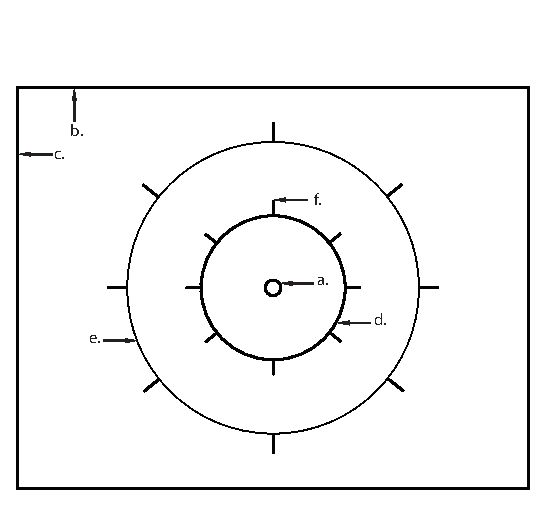
\includegraphics{std_skill_pattern_labeled}
\end{center}
\vspace{-20pt}
\caption{Riding Area Boundaries \label{fig:std_skill_pattern_labeled}}
\vspace{-10pt}
\end{figure}

\begin{enumerate}[a.]
\item Center circle (50cm diameter)
\item Long edge of riding area (faces judges)
\item Short edge of riding area
\item Inner circle (4m diameter) for circle figures
\item Outer circle (8m diameter) for line and figure eights.
\item Quarter and diagonal circle marks (length 1m) on the 4m and 8m circles.
Diagonals marked by going from corner to corner of the riding boundary.
\end{enumerate}


\subsection{Line Figure}
\begin{wrapfigure}{r}{0.35\textwidth}
\vspace{-35pt}
\begin{center}
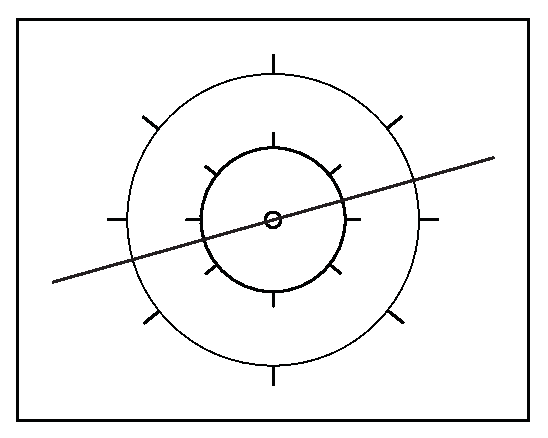
\includegraphics[width=0.33\textwidth]{std_skill_line_figure}
\end{center}
\vspace{-20pt}
\caption{Line Figure\label{fig:std_skill_line_figure}}
\vspace{-10pt}
\end{wrapfigure}
Lines, circles and figure eights may be ridden in any direction.
Line figures start outside the large (8m) circle, cross the center circle, and continue outside the large circle.
The rider must be in position for the figure before the hub crosses over the outside edge of the line.
For seat drag figures where the seat is forward of the riding direction, the rider must be in position before the seat crosses the outside edge of the line.
The line should be straight.
Circles and figure eights can be started at any point, as long as the rider completes the figure by crossing over the starting point.

\subsection{Circle Figure}
\begin{wrapfigure}{r}{0.35\textwidth}
\vspace{-75pt}
\begin{center}
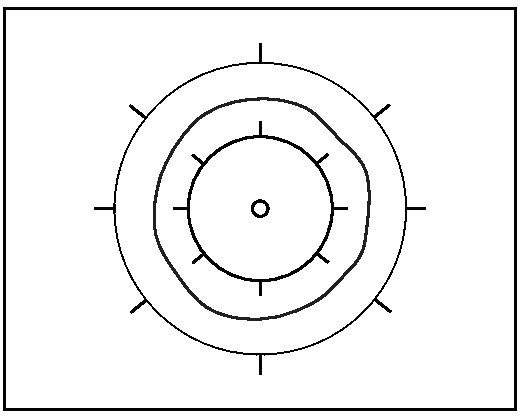
\includegraphics[width=0.33\textwidth]{std_skill_circle_figure}
\end{center}
\vspace{-20pt}
\caption{Circle Figure\label{fig:std_skill_circle_figure}}
\vspace{-10pt}
\end{wrapfigure}
Circle figures are ridden in the area between the 4m and 8m circle lines.
If the rider crosses the 4m line while performing the figure, the circle must be restarted from the point where the rider re-crosses to the outside of the 4m circle.
Crossing the 8m line does not invalidate the figure.
Circle figures should be as round as possible.

\subsection{Figure Eight}
\begin{wrapfigure}{r}{0.35\textwidth}
\vspace{-45pt}
\begin{center}
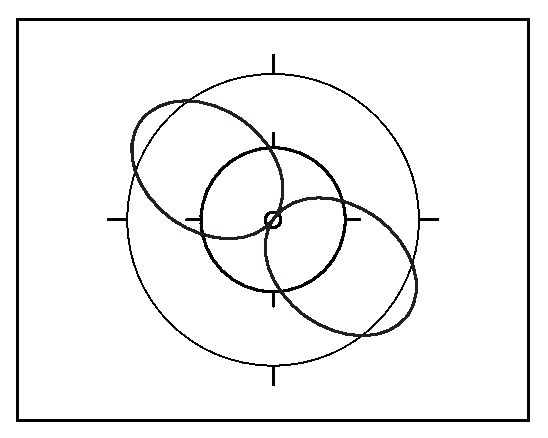
\includegraphics[width=0.33\textwidth]{std_skill_figure_eight}
\end{center}
\vspace{-20pt}
\caption{Figure Eight\label{fig:std_skill_figure_eight}}
\vspace{-10pt}
\end{wrapfigure}
The two circles making up the 8 should be the same size, and the orientation of the 8 can be in any direction.
The rider must pass outside the 8m circle on each end of the 8, and cross the center circle at the middle.
The two halves of the figure 8 must be circular, with diameters of at least 4m.

\section{Mounts, Transitions, Axis, Single And Counted Short Skills}
These are all collectively called ``non-riding skills''.
May be performed anywhere in the riding area unless stated differently in the description.

\section{Body Form}
Unless otherwise noted, each figure must be performed with riders sitting up straight with their arms stretched and horizontal.
Hands must be flat with palms down and fingers together.
Arms do not have to be straight out to the sides.
As long as arms are outstretched and horizontal, they may point in any direction.

\section{Dismounts}
All dismounts must be controlled, including the dismount at the end of the routine.
A controlled (intentional) dismount is where the rider comes to a stop and steps off the unicycle.
Dismounts executed otherwise will be considered unintentional.
A dismount occurs any time a rider touches the floor, except in skills where the rider is required to touch the floor, or when a foot on a pedal touches the floor.
The rules demand that the rider dismounts in a sportsmanlike manner at the end of the routine.
Failure to do so will result in a wave for insecure exit.

\section{Assisting Riders}
At international events it is forbidden for a rider to get verbal assistance or helping gestures from a person outside the riding area, since this is interference with the rider by an outside person.
At international events it is forbidden for a rider to use any props (including people) during the 3-minute routine.
Any competitor caught getting assistance (verbal or nonverbal) or using props may be disqualified from the competition.
Also, a rider may not look at the list of skills while performing the routine.
This includes skills written on the competitor's hand, a piece of paper or elsewhere.
Each occurrence of a competitor looking at a skills list will result in a wave.

\section{Standard Skill Judging Sheet}
Before competing in Standard Skill, each rider must fill out and turn in a judging sheet listing his or her routine.
This list includes the number, name, and point value of each figure to be performed in the routine, in the order in which they will be ridden.

\subsection{Skills To Be Used}
The maximum number of figures allowed is 18.
Of those 18 figures, no more than 12 may be other than a riding skill.
Skills with numbers 101 and higher are limited to a maximum of 12.
If a rider only chooses 12 skills for the whole routine, it is allowed for all of these to be non-riding skills.

\textbf{Note:} Each figure number may appear only once on the judging sheet.
This means that, for example, if a rider uses figure 15 b, he or she may not use 15 a, c, d, e, f, g, or h.

\subsection{Skill Order}
The 18 figures must be performed in the exact same order as they appear on the judging sheet.
Figures left out according to their order on the judging sheet will be devaluated 100\%.
This devaluation remains, even if the figure is performed later in the routine.
\textbf{Example:} The skills on a judging sheet are: wheel walk, one-foot, idle, riding backwards.
The rider does the wheel walk, skips the one-foot and idle, then performs the riding backwards, followed by the one-foot and the idle.
The technical judge will mark both the 1-ft and idle with a 100\% devaluation.

\subsection{Filling Out Judging Sheet}
The completed judging sheet must be sent in before the deadline date set by competition organizers.
When filling out the sheet, each figure name must be written out exactly as it appears on the Standard Skill List, with no further abbreviations.
Figure numbers, letters, and point values must be included, and the total Difficulty score (total points for all figures in the routine) must be filled in.
The judges have to check the judging sheets and, if possible in contact with the competitor, correct any mistakes.
Any disadvantage resulting from filling out a judging sheet incorrectly will be at the competitor's expense, and will not be valid grounds for protest.
Judging sheets, once checked and approved for competition, cannot be changed.

\subsection{Competitor and Judging Forms}
If available to the organizers, a computer database should be used to generate forms for both the competitor and the judges, and then be used to calculate the scores.
Either the Writing Judge Form or the traditional Standard Skill Form is required for judging.
The other forms are suggested to help both the competitors and judges.
Suggested forms are: 
\begin{itemize}
\item \textbf{Competitor Form:} Skill Order, Figure number and letter, Description, Score, and Skill Definition.
\item \textbf{Standard Skill Form:} Skill Order, Figure number and letter, Description, Score, and areas to mark 50/100\% technical devaluations and the ~ / + 0 execution devaluations.
An area at the bottom should be included to write in the names of the three judges.
An area at the bottom should also be included to help in manual scoring of the routines.
\item \textbf{Writing Judge Form:} Skill Order, Figure number and letter, Description, Score, and areas to mark 50/100\% technical devaluations and the ~ / + 0 execution devaluations.
An area at the bottom should be included to write in the names of the three judges.
\item \textbf{Difficulty Judge Form:} Skill Order, Figure number and letter, Description, Score, Skill Definition, and area to mark 50/100\% technical devaluations.
The addition of the Skill Definition can help the judge if there is clarification needed for the correct execution of the skill.
\item \textbf{Execution Judge Form:} Skill Order, Figure number and letter, Description, Score, and area to mark the ~ / + 0 execution devaluations.
\end{itemize}

All three judging forms should have grey shading to indicate the relative speed of the skills.
No shading would indicate a slower skill (typically all riding skills), a light grey indicates skills that are quicker than the riding skills (most of the counted short skills), and a dark grey indicates skills that are very quick.
This will help the judges estimate how quickly they must watch for new skills.

\chapter{Standard Skill Judging}

\section{Judging Panel \label{sec:freestyle_std-judging-panel}}
There will be 1 Chief Judge, 2 Difficulty Judges, 2 Execution Judges, 2 Writing Judges, and 1 Timer.
The judging panel will be divided into two judging units, each consisting of one Difficulty, one Execution, and one Writing Judge.
The judges will be appointed to the functions Writer, Execution, and Difficulty, respectively in order of their experience.
At Unicons, all judges for the Expert groups must have previous Unicon judging experience.

\section{Operation Of The Judges}
While the Difficulty and Execution Judges watch the routine, the Writing Judge reads the names of the figures from the list.
The Difficulty Judge indicates if a skill was fully completed, or the reduction percentage if it was not.
The Execution Judge indicates the execution mistakes using symbols, as described below.
The Writer writes down the verbal remarks of both judges on the judging sheet.
For this reason, the Writer is seated between the other two judges.
The position of the judging table must be so that all judges have a clear view of the entire riding area.
There must be enough space between the two judging units to ensure their working independently of each other.

A video of the performance may be reviewed if there are discrepancies in judge scores, or if a judge is in doubt about one or more of his/her scores.
When time allows, video can be reviewed by approval of the Chief Judge.
The Chief Judge should prearrange for routines to be recorded, but this is not a mandatory requirement.

Alternatively, to speed up the competition and judging, video cameras should be used to record the competition.
There must be at least two cameras, one on each of the two corners.
A third camera in the center is also good for a backup.
The recordings should be downloaded to a computer in approximately groups of ten competitors.
The judges will all be in a separate viewing area to watch the videos and make their scores.

\section{Difficulty Devaluations}

\subsection{Skill Verification}
Every figure on the judging sheet must be executed according to its description in the Standard Skill List.
If a performed figure does not correspond with the entry on the judging sheet, 100\% is devaluated.

\subsection{Technical Mistakes}
If a technical mistake occurs during the execution of a skill, 50\% is devaluated.
Technical mistakes include but are not limited to the following: 
\begin{itemize}
\item Part of body other than one hand touching seat in seat out skills
\item Hand holding seat touching body in seat out skills
\item Free foot touching rotating part of unicycle in one foot skills
\item Legs not extended and/or toe not pointed for skills where the leg is quickly extended (including, but not limited to: wheel grab, crank idle kick, hop on wheel kick)
\end{itemize}

\subsection{Skill Completion \label{subsec:freestyle_difficulty-devaluations_skill-completion}}
Every figure on the judging sheet must be performed as entered, from start to finish, without the rider touching the floor, except where required to by the figure description.
This applies to all skills: riding skills (figures in lines, circles and 8's), transitions, axis skills, single and counted short skills, and mounts.

\begin{wrapfigure}{l}{0.35\textwidth}
\vspace{-25pt}
\begin{center}
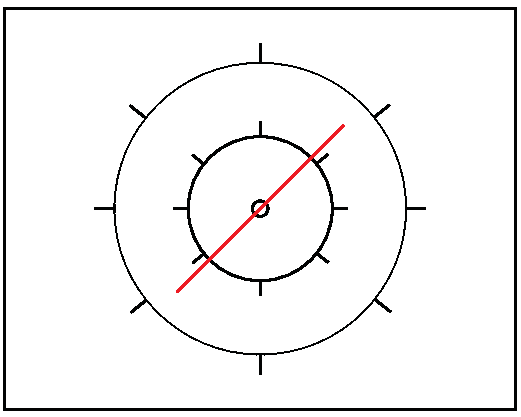
\includegraphics[width=0.33\textwidth]{std_skill_error_1}
\end{center}
\vspace{-20pt}
\caption{50\% Devaluation \label{fig:std_skill_error_1}}
\vspace{-5pt}
\begin{center}
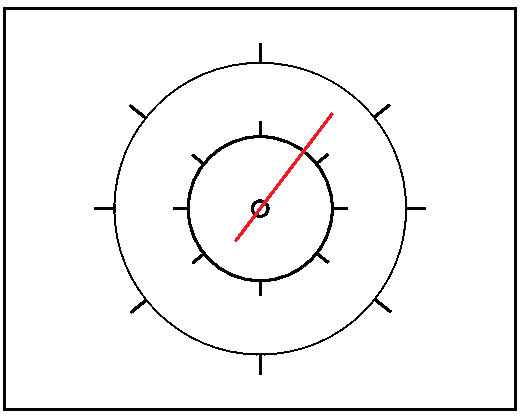
\includegraphics[width=0.33\textwidth]{std_skill_error_2}
\end{center}
\vspace{-20pt}
\caption{100\% Devaluation\label{fig:std_skill_error_2}}
\vspace{-25pt}
\end{wrapfigure}

\textbf{Riding Skills, Repetitive Axis Skills, and Counted Short Skills:} If a figure is broken off in the first half of its required execution, or performed for less than half of the required execution, 100\% is devaluated.
If a figure is broken off in the second half of the required execution, or performed for less than the required execution, 50\% is devaluated.

\textbf{Riding Skills:}
If a rider is not in position for a line figure before crossing the 8-meter circle, but is in position when crossing both 4-meter circle lines, 50\% is devaluated (see figure \ref{fig:std_skill_error_1}).
If the rider is in position but only crosses one edge of the 4-meter circle, 100\% is devaluated (see figure \ref{fig:std_skill_error_2}).

\textbf{Transitions and mounts:} Must finish in the end position (one revolution, $2 \frac{1}{2}$ hops, or $2 \frac{1}{2}$ idles) or 100\% is devaluated.
If the end position for a mount is not defined, must perform one revolution, OR $2 \frac{1}{2}$ hops, OR $2 \frac{1}{2}$ idles before stepping off the unicycle.

\textbf{Axis skills:} If the end position for a axis skill is not defined, must perform one revolution before stepping off the unicycle.
The ending position is not required to be the same as the starting position.

\textbf{Single Short Skills:} Unless otherwise defined in the skill description, the ending position is the same as the starting position.
Must finish in the end position (one revolution, $2 \frac{1}{2}$ hops, or $2 \frac{1}{2}$ idles) or 100\% is devaluated.
If the start and end position for a single short skill is not defined, must perform one revolution, $2 \frac{1}{2}$ hops, OR $2 \frac{1}{2}$ idles before stepping off the unicycle.

\subsection{Start Of Figures}
All figures start when the rider gets into the position required for that figure.

\subsection{Figure Order}
Figures left out according to their order on the judging sheet are devaluated 100\%.
This devaluation remains, even if the figure is performed afterward.

\subsection{Figure Patterns}
Riding figures that the rider doesn't attempt to be ridden as described in section \ref{subsec:freestyle_floor-markings-figure-shapes_riding-area-boundaries} should receive 100\% devaluation.

\textbf{Example:} The line figure is described as ``...start outside the large (8m) circle, cross the center circle, and continue outside the large circle''.
If the rider does not attempt to cross the center circle and performs the line circle completely outside the 4m circle, then 100\% is devaluated.

\section{Execution Devaluations}

\subsection{Wave (~) = -0.5 Point}
A wave is scored once per skill for each of the following execution mistakes listed below.
More than one wave can be applied to each skill, but if a rider makes the same mistake twice during one skill, they should only receive one wave.

\textbf{Example:} During wheel walking, a rider may have jerky body movements and fingers not together at the beginning - two waves should be applied.
If the rider then smoothly wheel walks for a while and then has jerky body movements again, a third wave should not be applied.
\begin{itemize}
\item insecure entrance or exit 
\item cramped, insecure execution 
\item jerky body movements 
\item not sitting up straight 
\item fingers not together 
\item free leg not stretched, toes not pointed 
\item waving arms 
\item jerky pedal movement 
\item line not straight 
\item circle not round 
\item crossing the 4 m circle when performing a skill in a circle 
\item failure to cross center circle in line or figure 8 
\item circles of figure 8 not the same size 
\item pedal, or foot on pedal touching floor 
\item wandering spin or pirouette 
\item circle size exceeds 1 meter diameter in a spin 
\item going outside riding area boundary 
\item looking at the standard skill order 
\item arms not stretched 
\item arms not horizontal 
\item palms not down 
\item arms touching the body during seat out skills
\end{itemize}

\subsection{Line (/) = - 1 Point}
A line is scored every time loss of control occurs.
Loss of control includes:
\begin{itemize}
\item loss of proper body form 
\item breaking off and restarting a skill 
\item loss of proper body form before or after transitions
\end{itemize}

\subsection{Cross (+) = - 2 Points}
A cross is scored each time an unintentional dismount occurs with the competitor landing on his or her feet without the unicycle being dropped.

\subsection{Circle (0) = - 3 Points}
A circle is scored each time an unintentional dismount occurs with a part of the rider other than his or her feet touching the floor (hand, knee, rear, etc.) or with the unicycle being dropped.
Seat drag skills only have this score applied if a part of the rider other than the feet touches the floor.

\subsection{Applying Lines, Circles, Crosses}
Lines, circles and crosses are scored every time they occur during and between all skills, whether entered on the score sheet or not.
Only the highest applicable devaluation symbol shall be imposed per execution mistake.
Most waves are not scored if they occur between skills listed on the judging sheet.
Waves can only be scored between skills if they are unrelated to body form.

\textbf{Example:} A competitor will not get a wave if the competitor's arms are not in proper form between skills listed on the judging sheet, but a competitor will get a wave for exceeding the riding area boundary.

\section{Totaling Scores}
After the routine is finished, the percentages and symbols from the judges are converted into numbers.
These numbers are subtracted from the rider's starting score.
Then, the scores of the two judging units are added together and divided by two to get the finishing score of a competitor.
The winner in the Standard Skill event is the competitor with the highest score.
If more than one competitor have the same score, placing is decided by the highest Execution score.
If those scores are also the same, the competitors receive tie scores.
